\section{Punto de Vista de Cooperación de Actor}


\subsection{Modelo de Cooperación de Actor}
\begin{figure}[h!]
	\centering
	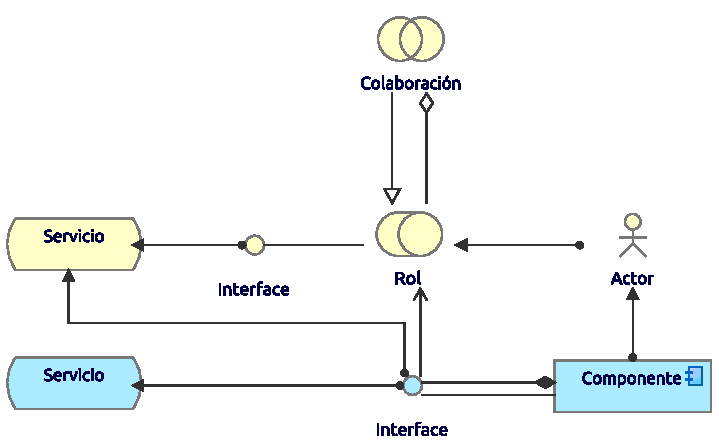
\includegraphics[width=.6\linewidth]{imgs/modelo/CoopActor.pdf}
	\caption{Modelo Cooperacion de Actor}
\end{figure}

El punto de vista de cooperación de actor establece las colaboraciones que existen internamente y externamente sobre un actor o rol de la organización con el fin de mostrar de qué manera interactuan e interfiere con el actor en cuestión. Por medio de interfaces  que comunican los entes del exterior y el interior de la organización con el actor o rol.

\newpage
\subsection{Caso  de Cooperación de Actor}
\begin{figure}[h!]
	\centering
	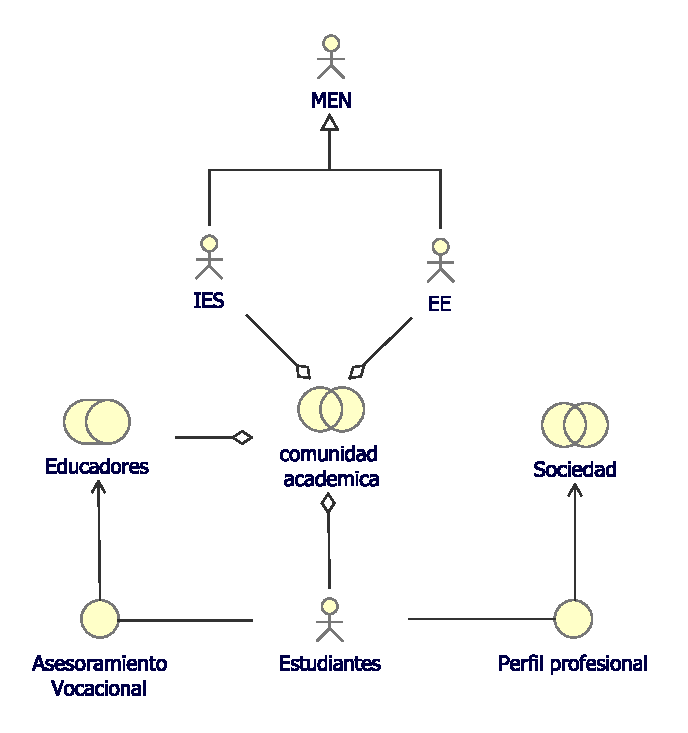
\includegraphics[width=.8\linewidth]{imgs/caso/negocio/coperacion_actor.pdf}
	\caption{Caso Cooperacion de Actor}
\end{figure}

Para nuestro objeto de estudio en relación al punto de vista de colaboración de actor tenemos como actor principal a los estudiantes aquellos que colaboran en la comunidad académica y hacen parte de las IES y EE que son regidas por el Ministerio de Educación. Por otro lado tenemos el rol de educador que hace parte de la comunidad y que puede ayudar a guiar en parte la vocación que construirá en un futuro el estudiante. Los estudiantes contribuirán en la sociedad gracias a su perfil que se ha formado durante sus años de estudio y que permitirán a las empresas apoderarse de estos individuos y así lograr mejores avances que colaboren en su entidad y por tanto a la sociedad misma.